\documentclass[12pt, a4paper]{article}

% --- PAQUETES ---
\usepackage[utf8]{inputenc}
\usepackage[T1]{fontenc}
\usepackage[spanish]{babel}
\usepackage{geometry}
\geometry{a4paper, margin=2.5cm}
\usepackage{setspace}
\usepackage{csquotes}
\usepackage{graphicx}
\usepackage{caption}

% Ruta a la carpeta de imágenes
\graphicspath{ {./images/} }

% --- BIBLIOGRAFÍA ESTILO APA 7 ---
\usepackage[
    backend=biber,
    style=apa,
    sorting=nyt
]{biblatex}

\DefineBibliographyStrings{spanish}{
  bibliography = {Referencias},
  references = {Referencias},
}
\addbibresource{referencias.bib}

% --- HIPERVÍNCULOS ---
\usepackage{hyperref}
\hypersetup{
    colorlinks=true,
    linkcolor=black,
    filecolor=magenta,
    urlcolor=blue,
    citecolor=black,
}


\begin{document}

% --- PORTADA (ESTILO INSTITUTO NACIONAL) ---
\begin{titlepage}
    \centering
    % Logo del Colegio
    
\includegraphics[width=3cm]{IN.png}\\[2cm]
    
    \large
    \textbf{Instituto Nacional José Miguel Carrera} \\
    % Puedes añadir el departamento aquí si lo necesitas
    % \textbf{Departamento de Historia y Ciencias Sociales}
    
    \vspace{2.5cm}
    \rule{\linewidth}{0.5mm}
    \vspace{0.4cm}
    
    \Huge
    \textbf{Desafíos para la Democracia en Chile: Un Análisis de la Percepción Ciudadana sobre Seguridad y Migración}
    
    \vspace{0.4cm}
    \rule{\linewidth}{0.5mm}
    
    \vspace{3cm}
    
    % Puedes añadir el nombre de la asignatura si quieres
    % \Large
    % \textbf{Educación Ciudadana}
    
    \vfill % Empuja el contenido hacia abajo
    
    \large
    \begin{tabular*}{\textwidth}{l @{\extracolsep{\fill}} r}
        \textbf{Autores:} & \textbf{Curso:} \\
        Felipe Colli & 4°H \\
        Benjamin Fernandez & \\
        Martin Valdenegro & \\
        Luciano Arevalo & \\
    \end{tabular*}
    
    \vspace{1.5cm}
    
    \large{\today} % Fecha de compilación
    
\end{titlepage}


% --- CONFIGURACIÓN E ÍNDICE ---
\onehalfspacing
\pagestyle{plain}
\tableofcontents
\newpage

% --- INTRODUCCIÓN ---
\section*{Introducción}
\addcontentsline{toc}{section}{Introducción}

La seguridad pública constituye un pilar fundamental para el desarrollo y la estabilidad de cualquier democracia. No solo representa una de las principales responsabilidades del Estado, sino que también es una condición esencial para que los ciudadanos puedan ejercer plenamente sus libertades y derechos. Cuando la percepción de inseguridad aumenta, la confianza en las instituciones se debilita y la cohesión social se ve amenazada. En el contexto chileno reciente, este tema ha escalado hasta convertirse en una de las preocupaciones más apremiantes para la ciudadanía, dominando el debate público y la agenda política.

Dentro de este complejo debate, el fenómeno migratorio ha emergido como un elemento de alta visibilidad, frecuentemente vinculado en el discurso público al aumento de la delincuencia. Como grupo, hemos elegido este desafío democrático por su alta relevancia actual y su impacto directo en la convivencia social. La consolidación de esta narrativa, sin un análisis basado en evidencia, presenta un riesgo para la democracia al poder fomentar la estigmatización de colectivos vulnerables y presionar por la formulación de políticas públicas basadas más en el temor que en datos objetivos.

El objetivo principal de este informe es, por tanto, analizar de manera objetiva la percepción ciudadana en torno a la seguridad y su posible relación con el fenómeno migratorio en Chile. Para llevar a cabo esta investigación, se diseñó y aplicó una encuesta online a 24 personas de diversas comunas, con el fin de recoger datos directos sobre sus experiencias, opiniones y las fuentes que moldean su visión. En las siguientes páginas, se presentará un análisis detallado de los datos recopilados y se contrastarán estos hallazgos sobre la percepción pública con datos oficiales de instituciones gubernamentales, buscando ofrecer una visión integral y fundamentada de este crítico desafío democrático.
\newpage

% --- DESARROLLO ---
\section{Desarrollo}
\subsection{Contexto: Seguridad y Migración en Cifras}
Para analizar de manera rigurosa la percepción ciudadana, es fundamental contextualizarla con los datos oficiales que describen la situación de la seguridad y la migración en Chile. Estos datos, provenientes de instituciones gubernamentales y de la sociedad civil, proporcionan un marco de referencia que permite entender la magnitud de los fenómenos y la posible brecha entre la percepción y la realidad estadística.

En materia de seguridad, la Encuesta Nacional Urbana de Seguridad Ciudadana (ENUSC) 2023, publicada por el INE, revela un panorama de alta preocupación \autocite{INE2024enusc}. Según este informe, un 90,6\% de la población percibe que la delincuencia en el país ha aumentado, cifra histórica que evidencia un temor masivo y generalizado. Este miedo tiene consecuencias directas: un 42,4\% de las personas reporta haber dejado de salir en ciertos horarios por la noche en su propio barrio, demostrando una alteración significativa de la vida cotidiana por causa de la inseguridad.

Paralelamente, es crucial dimensionar y caracterizar el fenómeno migratorio. Según la Estimación de Población Extranjera Residente 2023, publicada por el INE y el SERMIG, en Chile residen 1.773.522 personas extranjeras, lo que representa un 8,7\% de la población total del país \autocite{INE2024estimacion}. Es fundamental comprender el perfil de esta población: de acuerdo con la Encuesta de Caracterización de la Población Migrante 2022 \autocite{SERMIG2023encuesta}, sus principales motivos para migrar a Chile fueron laborales (64,9\%) y de reunificación familiar (19,8\%), lo que perfila una migración orientada principalmente a la búsqueda de oportunidades y proyectos de vida.

Para analizar la relación entre este fenómeno y la delincuencia, es imprescindible recurrir a los datos del sistema judicial. Cifras consolidadas del Ministerio Público para 2023 indican que del total de personas imputadas por la comisión de delitos a nivel nacional, solo un 6,2\% correspondía a personas de nacionalidad extranjera \autocite{MP2023}. Este dato es fundamental, pues muestra que la participación de extranjeros en delitos es, en términos proporcionales, inferior a su representación en la población general del país (8,7\%). Este hallazgo es reforzado por análisis del Servicio Jesuita a Migrantes (SJM Chile), que, basándose en datos del Poder Judicial, señala que el 84\% de las personas extranjeras imputadas no cuenta con antecedentes penales previos en Chile y que los migrantes tienen el doble de probabilidades de ser víctimas de delitos que de ser victimarios \autocite{SJM2024seguridad}.

\subsection{Análisis de Resultados: Encuesta sobre Percepción Ciudadana}
Nuestra encuesta, aplicada a 24 personas de diversas comunas, buscó capturar las percepciones directas de la ciudadanía sobre estos temas. A continuación, se presentan los hallazgos más relevantes.

\subsubsection*{Hallazgo 1: La Geografía del Miedo y el Refugio en lo Privado}
Un primer resultado contundente es la drástica diferencia en la percepción de seguridad entre el espacio privado y el público. Como se observa en el Gráfico \ref{fig:seguridad}, el hogar es percibido como el único espacio verdaderamente seguro, mientras que los espacios públicos, especialmente aquellos vinculados al transporte, son focos de alta inseguridad. El ``Paradero de micro/colectivo'' y la ``Micro/Metro'' son los lugares peor evaluados. Las respuestas abiertas refuerzan este dato; un participante señaló sentirse inseguro en el paradero ``por la falta de iluminación y la soledad, que lo convierten en un blanco fácil para asaltos''. Esta percepción transforma el tránsito cotidiano en una experiencia de constante vulnerabilidad.

\begin{figure}[!htbp]
	\centering
	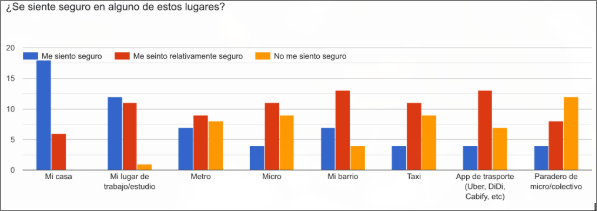
\includegraphics[width=\textwidth]{grafico_seguridad.png}
	\caption{Nivel de Seguridad por Lugar.}
	\label{fig:seguridad}
\end{figure}

\subsubsection*{Hallazgo 2: Una Visión Multifactorial sobre las Causas de la Delincuencia}
Al consultar sobre los principales factores que influyen en la delincuencia actual, los encuestados no apuntaron a una única causa, sino a un conjunto de problemas sistémicos. Como detalla el Gráfico \ref{fig:factores}, las causas más mencionadas fueron ``Leyes demasiado blandas'', ``Falta de presencia policial'', ``Narcotráfico'' y ``Falta de oportunidades económicas y laborales''. La ``Inmigración descontrolada'' fue seleccionada como un factor relevante, pero se situó por debajo de estas problemáticas estructurales del país. Este hallazgo es crucial, pues sugiere que, si bien una parte de la ciudadanía establece un vínculo entre ambos fenómenos, lo enmarca dentro de una crisis de seguridad más amplia y compleja.

\begin{figure}[!htbp]
	\centering
	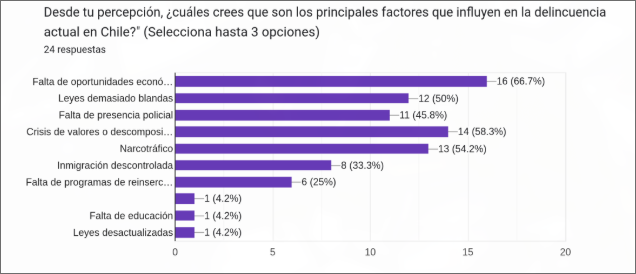
\includegraphics[width=\textwidth]{grafico_factores.png}
	\caption{Factores que Influyen en la Delincuencia.}
	\label{fig:factores}
\end{figure}

\subsubsection*{Hallazgo 3: Crítica Generalizada a la Gestión Migratoria del Estado}
Existe un consenso casi unánime en la evaluación negativa de la gestión estatal del fenómeno migratorio. En una escala de 1 a 5, la calificación promedio fue extremadamente baja, con la mayoría de las respuestas concentradas en las opciones 1 (``Muy mala'') y 2. Esto denota una profunda insatisfacción ciudadana con la capacidad de las instituciones para planificar, regular y gestionar la llegada de población extranjera, lo que puede ser un factor que alimenta la percepción de ``descontrol'' mencionada en la pregunta anterior.

\subsubsection*{Hallazgo 4: El Rol Central de las Redes Sociales en la Formación de Opinión}
Para comprender el origen de estas percepciones, se preguntó a los encuestados sobre sus principales fuentes de información. Como muestra el Gráfico \ref{fig:fuentes}, las ``Redes sociales'' (Facebook, TikTok, etc.), las ``Conversaciones con cercanos'' y la ``Experiencia personal'' superaron a los medios de comunicación tradicionales como la televisión o la prensa digital. Este dato es de suma importancia, ya que indica que la opinión pública sobre un tema tan sensible se construye en gran medida a través de algoritmos y círculos de confianza, donde la información no siempre es verificada y las narrativas emocionales pueden tener un mayor impacto que los datos oficiales.

\begin{figure}[!htbp]
	\centering
	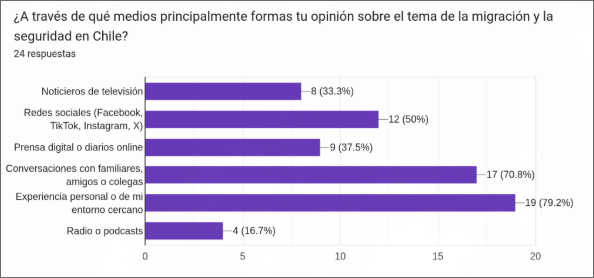
\includegraphics[width=\textwidth]{grafico_fuentes.png}
	\caption{Principales Fuentes de Información.}
	\label{fig:fuentes}
\end{figure}

% --- DISCUSIÓN ---
\section*{Discusión: La Brecha entre Percepción y Realidad Estadística}
\addcontentsline{toc}{section}{Discusión: La Brecha entre Percepción y Realidad Estadística}
Al cruzar los datos oficiales con los resultados de nuestra encuesta, emerge una clara disonancia entre la percepción ciudadana y la realidad estadística. Mientras que la ENUSC 2023 confirma que el temor es un sentimiento generalizado (90,6\%), nuestra investigación sugiere que este temor es canalizado, en parte, hacia el colectivo migrante.

El hallazgo clave reside en la comparación de cifras: mientras que los datos del Ministerio Público muestran que la participación de extranjeros en delitos (6,2\%) es incluso menor a su peso demográfico (8,7\%), la percepción ciudadana captada en nuestra encuesta sí establece un vínculo relevante entre ``inmigración descontrolada'' y delincuencia. Esta brecha no surge de la nada. Se alimenta de tres factores identificados en este estudio:
\begin{enumerate}
	\item Una crisis de seguridad real que genera un alto nivel de temor en la población.
	\item Una evaluación negativa de la gestión estatal, que refuerza la idea de ``descontrol'' y falta de autoridad.
	\item Un ecosistema informativo dominado por redes sociales, que facilita la rápida viralización de narrativas que asocian el delito a un rostro visible, como el del migrante.
\end{enumerate}

El impacto de esta disonancia es un desafío directo para la democracia. Fomenta la estigmatización de un grupo completo de la población, dificulta la creación de políticas de integración efectivas y puede llevar a la adopción de medidas punitivas populistas que, basadas en una percepción distorsionada, no resuelven las causas de fondo del problema delictual, como son la desigualdad, la falta de oportunidades o la debilidad de las instituciones.

% --- CONCLUSIÓN ---
\section*{Conclusión}
\addcontentsline{toc}{section}{Conclusión}

Esta investigación se propuso analizar la percepción ciudadana sobre la seguridad y su relación con el fenómeno migratorio, para comprender uno de los desafíos más complejos de la democracia chilena actual. A través de la aplicación de una encuesta y su contraste con datos oficiales, el estudio ha llegado a conclusiones significativas. Se confirmó que la alta percepción de inseguridad, reportada por la ENUSC 2023, es una realidad palpable para los encuestados, quienes identifican los espacios públicos como los principales focos de temor. Sin embargo, nuestro hallazgo central reside en la existencia de una brecha considerable entre la percepción pública y la realidad estadística: si bien los ciudadanos vinculan la ``inmigración descontrolada'' con la crisis de seguridad, los datos del Ministerio Público muestran que la participación de extranjeros en delitos es proporcionalmente inferior a su representación en la población total.

El verdadero desafío democrático, por tanto, no radica únicamente en el control del delito, sino en la gestión de esta disonancia. Nuestros resultados sugieren que esta brecha es alimentada por una evaluación muy negativa de la gestión estatal y un ecosistema informativo dominado por las redes sociales, donde las narrativas emocionales pueden prevalecer sobre la evidencia. El impacto de esto es profundo: se corre el riesgo de estigmatizar a colectivos completos, erosionar la cohesión social y promover políticas públicas punitivas que, al estar basadas en una percepción distorsionada, no abordan las causas de fondo que los propios encuestados identificaron, como la debilidad de las leyes y la falta de oportunidades.

Como grupo, la realización de este informe nos ha proporcionado un aprendizaje fundamental sobre el rigor que exige la investigación social. Comprendimos la importancia de formular preguntas neutrales para evitar sesgos y la necesidad de contrastar siempre las opiniones con datos verificables. Si bien nuestro estudio tiene la limitación de una muestra acotada que no es estadísticamente representativa de todo el país, nos ha permitido ilustrar con claridad la complejidad de un fenómeno donde el temor, la realidad y la información interactúan de manera constante. Finalmente, este trabajo reafirma la idea de que una democracia sana requiere no solo ciudadanos seguros, sino también bien informados.

\newpage
% --- IMPRIMIR REFERENCIAS ---
\printbibliography

\end{document}
